\documentclass[12pt,a4paper]{article}

\usepackage[margin=0.95in, headheight=15pt]{geometry}
\usepackage{graphicx}
\usepackage{amsmath}
\usepackage{amssymb}
\usepackage{float}
\usepackage{titlesec}
\usepackage{setspace}
\usepackage{hyperref}
\usepackage{booktabs}
\usepackage{array}
\usepackage{xcolor}
\usepackage{colortbl}
\usepackage{enumitem}
\usepackage{listings}
\usepackage{tikz}
\usepackage{pgfplots}
\pgfplotsset{compat=1.18}
\usetikzlibrary{shapes.geometric, arrows.meta, positioning, fit,
                backgrounds, calc, decorations.pathreplacing}
\usepackage{caption}
\usepackage{subcaption}
\usepackage{fancyhdr}
\usepackage{lastpage}
\usepackage{tcolorbox}
\tcbuselibrary{skins}
\usepackage{multicol}

% ── Colours ────────────────────────────────────────────────────────────────
\definecolor{primary}{RGB}{102,126,234}
\definecolor{accent}{RGB}{6,182,212}
\definecolor{dark}{RGB}{15,52,96}
\definecolor{headerbg}{RGB}{26,26,46}
\definecolor{codegreen}{RGB}{46,160,67}
\definecolor{codegray}{RGB}{100,100,100}
\definecolor{codepurple}{RGB}{118,75,162}
\definecolor{lightblue}{RGB}{200,215,255}
\definecolor{placeholderbg}{RGB}{240,242,250}
\definecolor{placeholderborder}{RGB}{180,195,240}

% ── Page style ─────────────────────────────────────────────────────────────
\pagestyle{fancy}
\fancyhf{}
\rhead{\textcolor{codegray}{\small AsanaAI — CELBC608 DSL Sem VI}}
\lhead{\textcolor{codegray}{\small Yoga Pose Recognition · Transfer Learning · Grad-CAM}}
\rfoot{\textcolor{codegray}{\small Page \thepage\ of \pageref{LastPage}}}
\renewcommand{\headrulewidth}{0.4pt}
\renewcommand{\footrulewidth}{0.4pt}

% ── Typography ─────────────────────────────────────────────────────────────
\setstretch{1.18}
\titleformat{\section}{\large\bfseries\color{dark}}{\thesection}{1em}{}
  [\vspace{-0.3em}\rule{\linewidth}{0.6pt}]
\titleformat{\subsection}{\normalsize\bfseries\color{primary}}{\thesubsection}{1em}{}
\titleformat{\subsubsection}{\normalsize\bfseries\color{codegray}}{\thesubsubsection}{1em}{}
\titlespacing*{\section}{0pt}{8pt}{4pt}
\titlespacing*{\subsection}{0pt}{5pt}{2pt}

% ── Code listing style ─────────────────────────────────────────────────────
\lstset{
  language=Python,
  basicstyle=\ttfamily\scriptsize,
  keywordstyle=\color{codepurple}\bfseries,
  commentstyle=\color{codegreen},
  stringstyle=\color{accent},
  numberstyle=\tiny\color{codegray},
  numbers=left,
  breaklines=true,
  frame=single,
  rulecolor=\color{lightblue},
  backgroundcolor=\color{gray!5},
  captionpos=b,
  tabsize=4,
  showstringspaces=false,
  xleftmargin=1.5em,
  framexleftmargin=1.5em,
}

% ── Screenshot placeholder command (taller: 4.5cm) ─────────────────────────
\newcommand{\screenshotbox}[2]{%
  \begin{center}
  \setlength{\fboxsep}{0pt}%
  \fcolorbox{placeholderborder}{placeholderbg}{%
    \begin{minipage}[c][4.5cm]{\dimexpr\linewidth-2\fboxrule}%
      \centering
      \vfill
      {\color{primary}\textbf{\footnotesize #1}}\\[0.35em]
      {\color{codegray}\scriptsize #2}
      \vfill
    \end{minipage}%
  }%
  \end{center}%
}

% ── TikZ node styles ───────────────────────────────────────────────────────
\tikzset{
  block/.style={rectangle, rounded corners=4pt, draw=primary, fill=primary!10,
    text width=2.0cm, align=center, minimum height=0.85cm, font=\scriptsize},
  wideblock/.style={rectangle, rounded corners=4pt, draw=primary, fill=primary!10,
    text width=2.8cm, align=center, minimum height=0.85cm, font=\scriptsize},
  arrow/.style={-{Stealth[length=5pt]}, thick, color=dark},
  layer/.style={rectangle, rounded corners=3pt, draw=accent, fill=accent!12,
    text width=2.6cm, align=center, minimum height=0.75cm, font=\scriptsize},
  smlayer/.style={rectangle, rounded corners=3pt, draw=codepurple,
    fill=codepurple!10, text width=2.7cm, align=center,
    minimum height=0.7cm, font=\scriptsize},
  io/.style={trapezium, trapezium left angle=68, trapezium right angle=112,
    draw=accent, fill=accent!10, align=center, minimum height=0.8cm,
    text width=1.9cm, font=\scriptsize},
  decision/.style={diamond, draw=primary, fill=primary!10, aspect=2.2,
    align=center, font=\scriptsize},
  stepbox/.style={rectangle, rounded corners, draw=primary, fill=primary!8,
    text width=6cm, align=center, minimum height=0.85cm, font=\small},
}

% ══════════════════════════════════════════════════════════════════════════
% ── Title page ─────────────────────────────────────────────────────────────
\titleformat{\section}{\large\bfseries}{\thesection}{1em}{}
\titleformat{\subsection}{\normalsize\bfseries}{\thesubsection}{1em}{}

\title{\textbf{AsanaAI: Explainable Deep Learning System for Yoga Pose Recognition}}
\author{Shreyas Sawant 1023242 \\ Amit Singh 1023254 \\
\textit{Fr. C. Rodrigues Institute of Technology}}
\date{\today}

\begin{document}

\maketitle

% ── Abstract ───────────────────────────────────────────────────────────────
\begin{tcolorbox}[colback=primary!6, colframe=primary,
  title=\bfseries Abstract, fonttitle=\small, boxrule=0.8pt, arc=4pt]
\small\setstretch{1.2}
AsanaAI is a full-stack explainable deep-learning application for yoga pose classification
from still images and live webcam input. The system uses two-stage transfer learning on
MobileNetV2 trained with AdamW optimisation, MixUp regularisation, label smoothing,
gradient clipping, and post-hoc temperature calibration. Predictions are made interpretable
through Gradient-weighted Class Activation Mapping (Grad-CAM). The Streamlit interface
supports dataset upload (ZIP), live-epoch training, comprehensive evaluation (accuracy,
confusion matrix, per-class metrics, ROC/AUC), single-image inference, live webcam
pose assistance, and pose guidance cards across 16 yoga classes. Trained checkpoints,
class-name order, and calibration temperature are persisted and auto-loaded, removing
the need for redundant retraining.\\[3pt]
\textbf{Keywords:} Transfer learning, MobileNetV2, Grad-CAM, Streamlit, PyTorch,
explainable AI, temperature calibration, MixUp, two-stage fine-tuning, webcam inference.
\end{tcolorbox}

\newpage
{\small\tableofcontents}
\newpage

% ══════════════════════════════════════════════════════════════════════════
\section{Introduction}
% ══════════════════════════════════════════════════════════════════════════

Incorrect yoga posture is a common cause of preventable injury among beginners who
practise without instructor supervision. An AI classifier that gives rapid pose
identification and visual evidence of its reasoning can help fill this gap.

AsanaAI is built on three design pillars:
\begin{enumerate}[leftmargin=1.5em, label=\textbf{\arabic*.}, itemsep=1pt]
  \item \textbf{Robust classification} — Two-stage transfer learning with MobileNetV2
    achieves high accuracy on a dataset of 1920 images across 16 classes.
  \item \textbf{Visual interpretability} — Grad-CAM overlays show which body regions
    drove each prediction, building user trust and enabling qualitative checks.
  \item \textbf{Reproducibility and live access} — Checkpoint persistence, calibrated
    confidence, webcam input, and a Streamlit UI ensure consistent results across sessions.
\end{enumerate}

% ══════════════════════════════════════════════════════════════════════════
\section{Dataset Description}
% ══════════════════════════════════════════════════════════════════════════

\subsection{Class Set and Split}
The dataset is a curated subset of publicly available yoga posture images, organised
into 16 classes with a deterministic 80/20 physical train/val split.

\begin{table}[H]
\centering\small
\caption{Dataset class summary (1920 images total, 96 train + 24 val per class)}
\renewcommand{\arraystretch}{1.15}
\begin{tabular}{@{}llcc@{}}
\toprule
\textbf{Class} & \textbf{Sanskrit Name} & \textbf{Train} & \textbf{Val} \\
\midrule
\rowcolor{lightblue!30} Camel Pose          & Ustrasana                 & 96 & 24 \\
Crane Pose                                  & Bakasana                  & 96 & 24 \\
\rowcolor{lightblue!30} Eight-Angle Pose    & Astavakrasana             & 96 & 24 \\
Full Boat Pose                              & Navasana                  & 96 & 24 \\
\rowcolor{lightblue!30} King Dancer Pose    & Natarajasana              & 96 & 24 \\
Plow Pose                                   & Halasana                  & 96 & 24 \\
\rowcolor{lightblue!30} Sitting Half Spinal Twist & Ardha Matsyendrasana & 96 & 24 \\
child\_pose                                 & Balasana                  & 96 & 24 \\
\rowcolor{lightblue!30} cobra               & Bhujangasana              & 96 & 24 \\
cow pose                                    & Bitilasana                & 96 & 24 \\
\rowcolor{lightblue!30} downward\_dog       & Adho Mukha Svanasana      & 96 & 24 \\
plank                                       & Phalakasana               & 96 & 24 \\
\rowcolor{lightblue!30} seated\_forward\_bend & Paschimottanasana       & 96 & 24 \\
tree                                        & Vrikshasana               & 96 & 24 \\
\rowcolor{lightblue!30} triangle            & Trikonasana               & 96 & 24 \\
warrior                                     & Virabhadrasana I          & 96 & 24 \\
\midrule
\textbf{Total} & & \textbf{1536} & \textbf{384} \\
\bottomrule
\end{tabular}
\end{table}

\noindent The validation loader always uses \texttt{shuffle=False} to ensure deterministic,
reproducible metric computation. Train and val images are stored in separate physical
folder trees to prevent data leakage.

\subsection{EDA — Dataset Summary}
\screenshotbox{Screenshot: EDA Dashboard — Class Distribution \& Sample Images}{
  Insert screenshot of the EDA panel showing: (a) class-wise image count bar chart
  for all 16 train/val splits, (b) sample image grid (one image per class),
  and (c) augmentation preview of 6 random transforms applied to one image.}

% ══════════════════════════════════════════════════════════════════════════
\section{System Architecture and Design (Practical 4)}
% ══════════════════════════════════════════════════════════════════════════

\subsection{End-to-End System Pipeline}

\begin{figure}[H]
\centering
\resizebox{\linewidth}{!}{%
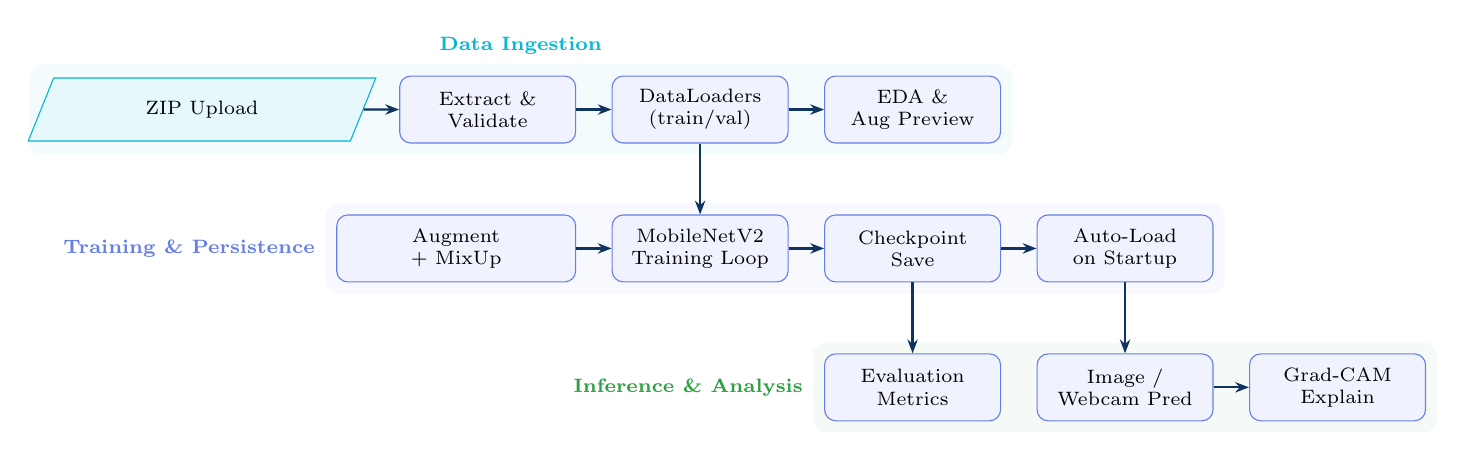
\begin{tikzpicture}[node distance=0.55cm and 0.4cm]
  % Row 1 — ingestion
  \node[io]                           (zip)     {ZIP Upload};
  \node[block, right=0.45cm of zip]   (extract) {Extract \&\\Validate};
  \node[block, right=0.45cm of extract](loaders){DataLoaders\\(train/val)};
  \node[block, right=0.45cm of loaders](eda)    {EDA \&\\Aug Preview};

  % Row 2 — training
  \node[block, below=0.9cm of loaders](train)  {MobileNetV2\\Training Loop};
  \node[wideblock, left=0.45cm of train](augment){Augment\\+ MixUp};
  \node[block, right=0.45cm of train] (save)    {Checkpoint\\Save};
  \node[block, right=0.45cm of save]  (autoload){Auto-Load\\on Startup};

  % Row 3 — inference
  \node[block, below=0.9cm of save]  (eval)    {Evaluation\\Metrics};
  \node[block, right=0.45cm of eval]  (pred)    {Image /\\Webcam Pred};
  \node[block, right=0.45cm of pred]  (gradcam) {Grad-CAM\\Explain};

  % Arrows
  \draw[arrow] (zip)--(extract);
  \draw[arrow] (extract)--(loaders);
  \draw[arrow] (loaders)--(eda);
  \draw[arrow] (loaders)--(train);
  \draw[arrow] (augment)--(train);
  \draw[arrow] (train)--(save);
  \draw[arrow] (save)--(autoload);
  \draw[arrow] (save)--(eval);
  \draw[arrow] (autoload)--(pred);
  \draw[arrow] (pred)--(gradcam);

  % Phase backgrounds
  \begin{scope}[on background layer]
    \node[fit=(zip)(extract)(loaders)(eda),
          fill=accent!5, rounded corners=5pt, inner sep=4pt,
          label=above:{\scriptsize\color{accent}\bfseries Data Ingestion}]{};
    \node[fit=(augment)(train)(save)(autoload),
          fill=primary!5, rounded corners=5pt, inner sep=4pt,
          label=left:{\scriptsize\color{primary}\bfseries Training \& Persistence}]{};
    \node[fit=(eval)(pred)(gradcam),
          fill=codegreen!5, rounded corners=5pt, inner sep=4pt,
          label=left:{\scriptsize\color{codegreen}\bfseries Inference \& Analysis}]{};
  \end{scope}
\end{tikzpicture}%
}
\caption{AsanaAI end-to-end system pipeline}
\label{fig:pipeline}
\end{figure}

\subsection{Model Architecture}

\subsubsection{Backbone — MobileNetV2}
MobileNetV2 uses inverted residual blocks with depthwise-separable convolutions,
giving strong feature extraction at low computational cost, which makes it suitable
for CPU-only lab machines. It is initialised with
\texttt{MobileNet\_V2\_Weights.DEFAULT} (ImageNet pre-training).

\subsubsection{Two-Stage Freezing Strategy}
All backbone parameters are frozen during head warm-up (epochs 1--9). From epoch 10
onward, feature blocks at index $\geq 16$ are selectively unfrozen with a lower
learning rate ($2\times10^{-5}$), allowing domain adaptation while keeping early
spatial filters intact.

\subsubsection{Custom Classification Head}
The original MobileNetV2 classifier is replaced with:

\begin{equation}
  \hat{y} = \text{Linear}_{128 \to K}\!\Bigl(
    \text{Dropout}_{0.3}\!\bigl(
      \text{ReLU}\!\bigl(
        \text{Linear}_{1280 \to 128}(\mathbf{z})
      \bigr)
    \bigr)
  \Bigr), \quad K = 16
\end{equation}

\begin{figure}[H]
\centering
\resizebox{0.52\linewidth}{!}{%
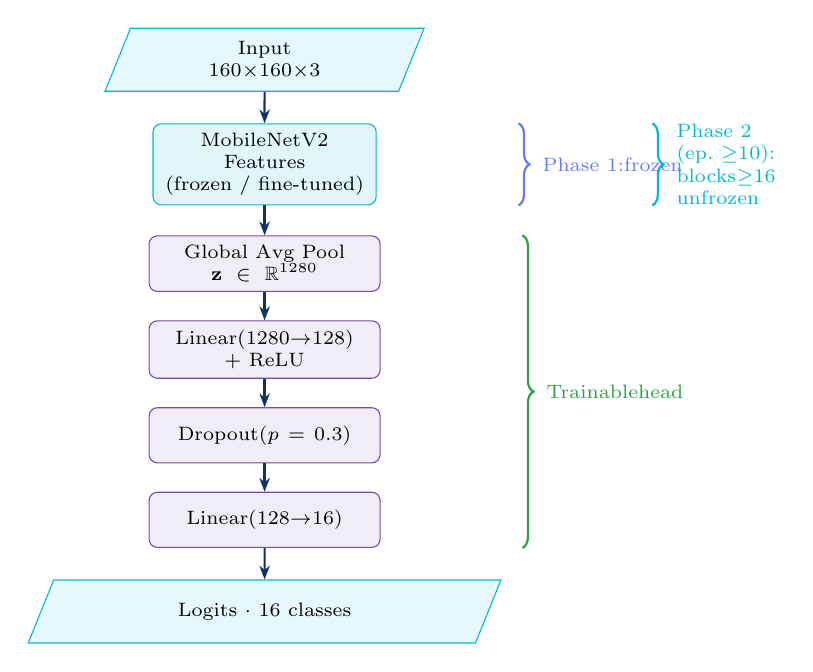
\begin{tikzpicture}[node distance=0.42cm]
  \node[io, text width=2.8cm] (input) {Input\\$160{\times}160{\times}3$};
  \node[layer, below=0.4cm of input] (feat)
    {MobileNetV2 Features\\(frozen / fine-tuned)};
  \node[smlayer, below=0.38cm of feat] (gap)  {Global Avg Pool\\$\mathbf{z}\in\mathbb{R}^{1280}$};
  \node[smlayer, below=0.36cm of gap]  (fc1)  {Linear($1280{\to}128$) + ReLU};
  \node[smlayer, below=0.36cm of fc1]  (drop) {Dropout($p=0.3$)};
  \node[smlayer, below=0.36cm of drop] (fc2)  {Linear($128{\to}16$)};
  \node[io, text width=2.8cm, below=0.4cm of fc2] (out) {Logits $\cdot$ 16 classes};

  \foreach \f/\t in {input/feat,feat/gap,gap/fc1,fc1/drop,drop/fc2,fc2/out}
    \draw[arrow] (\f)--(\t);

  % Brace: frozen phase
  \draw[decorate, decoration={brace,amplitude=4pt}, color=primary, thick]
    ([xshift=1.8cm]feat.north east)--([xshift=1.8cm]feat.south east)
    node[midway, right=5pt, font=\scriptsize, color=primary]{Phase 1:\\frozen};
  % Brace: trainable head
  \draw[decorate, decoration={brace,amplitude=4pt}, color=codegreen, thick]
    ([xshift=1.8cm]gap.north east)--([xshift=1.8cm]fc2.south east)
    node[midway, right=5pt, font=\scriptsize, color=codegreen]{Trainable\\head};
  % Brace: phase 2
  \draw[decorate, decoration={brace,amplitude=4pt}, color=accent, thick]
    ([xshift=3.5cm]feat.north east)--([xshift=3.5cm]feat.south east)
    node[midway, right=5pt, font=\scriptsize, color=accent, align=left]
      {Phase 2\\(ep.\ ${\geq}10$):\\blocks$\geq$16\\unfrozen};
\end{tikzpicture}%
}
\caption{Model architecture with two-phase training strategy (K = 16 output classes)}
\label{fig:arch}
\end{figure}

% ══════════════════════════════════════════════════════════════════════════
\section{Preprocessing, Augmentation and Training (Practical 4)}
% ══════════════════════════════════════════════════════════════════════════

\subsection{Transform Pipelines}

\begin{table}[H]
\centering\small
\caption{Training vs.\ validation transform pipelines}
\renewcommand{\arraystretch}{1.2}
\begin{tabular}{@{}p{3.4cm}p{4.6cm}p{3.8cm}@{}}
\toprule
\textbf{Transform} & \textbf{Training} & \textbf{Validation} \\
\midrule
\rowcolor{lightblue!20} Resize / Crop &
  RandomResizedCrop(160, scale 0.85--1.0) &
  Resize(184) then CenterCrop(160) \\
Flip & RandomHorizontalFlip ($p=0.5$) & None \\
\rowcolor{lightblue!20} Affine &
  Random $\pm10^{\circ}$, translate $4\%$, scale $\pm5\%$ & None \\
Colour & ColorJitter (br/ct 0.12, sat 0.08, hue 0.02) & None \\
\rowcolor{lightblue!20} Sharpness & RandomAdjustSharpness(1.3, $p=0.2$) & None \\
Normalise & ImageNet mean/std & ImageNet mean/std \\
\bottomrule
\end{tabular}
\end{table}

\noindent Validation images are never augmented to ensure fair, unbiased evaluation.

\subsection{MixUp Regularisation}
For the first 10 epochs, MixUp augmentation blends pairs of training images to reduce
overconfidence on the small dataset:

\begin{equation}
  \tilde{x} = \lambda x_i + (1-\lambda)x_j, \quad
  \mathcal{L}_\text{mix} = \lambda\mathcal{L}(f(\tilde{x}),y_i)
  + (1-\lambda)\mathcal{L}(f(\tilde{x}),y_j), \quad
  \lambda \sim \text{Beta}(0.2,\,0.2)
\end{equation}

MixUp is disabled from epoch 11 so the fine-tuning phase trains on clean samples.

\subsection{Training Hyperparameters}

\begin{table}[H]
\centering\small
\caption{Full training hyperparameter specification}
\renewcommand{\arraystretch}{1.2}
\begin{tabular}{@{}lll@{}}
\toprule
\textbf{Parameter} & \textbf{Value} & \textbf{Notes} \\
\midrule
\rowcolor{lightblue!20} Image size & $160\times160$ & Resize to 184, CenterCrop \\
Batch size & 12 & Balanced for CPU and GPU memory \\
\rowcolor{lightblue!20} Max epochs & 24 & With early stopping (patience = 6) \\
Optimizer (head) & AdamW, lr $5\times10^{-4}$ & Classifier head only \\
\rowcolor{lightblue!20} Optimizer (fine-tune) & AdamW, lr $2\times10^{-5}$ & Blocks $\geq16$ + head \\
Weight decay & $10^{-4}$ & Both phases \\
\rowcolor{lightblue!20} LR scheduler & ReduceLROnPlateau & factor 0.5, patience 1, min $10^{-6}$ \\
Label smoothing & $0.05$ & Applied in CrossEntropyLoss \\
\rowcolor{lightblue!20} Gradient clipping & 1.0 & Clips gradient norm \\
MixUp $\alpha$ & 0.2 & Epochs 1--10 only \\
\rowcolor{lightblue!20} Class weighting & Auto & Enabled if imbalance ratio $\geq 1.5$ \\
Fine-tune trigger & Epoch 10 & Unfreeze blocks $\geq 16$ \\
\bottomrule
\end{tabular}
\end{table}

\subsection{Loss Function}
Label-smoothed cross-entropy reduces overconfident predictions on the limited dataset:

\begin{equation}
  \mathcal{L}_\text{LS} = (1-\varepsilon)\,\mathcal{L}_\text{CE}(p,y)
  + \frac{\varepsilon}{K}\sum_{k=1}^{K}\mathcal{L}_\text{CE}(p,k),
  \quad \varepsilon=0.05,\; K=16
\end{equation}

When the class imbalance ratio reaches $\geq 1.5$, per-class weights $w_k = \bar{N}/N_k$
are applied automatically. An optional \texttt{WeightedRandomSampler} for oversampling
minority classes is also available via a UI toggle.

\subsection{Post-hoc Temperature Calibration}
After training, a temperature scalar $T$ is found on validation logits via grid search
over $T\in[0.5,\,2.5]$ (41 steps) to minimise negative log-likelihood:

\begin{equation}
  T^* = \arg\min_{T}\;\frac{1}{N}\sum_{i=1}^{N}
  -\log\,\text{softmax}\!\left(\frac{z_i}{T}\right)_{\!y_i}
\end{equation}

Calibrated probabilities at inference time are $p_k = \text{softmax}(z/T^*)_k$.
The temperature value is saved in \texttt{training\_history.json} and restored on load.
For the trained model, the imbalance ratio was 8.15 (class weighting enabled),
and the best validation accuracy reached \textbf{87.6\%} at epoch 21.

\subsection{Training Results — Learning Curves}
\screenshotbox{Screenshot: Training Learning Curves}{
  Insert screenshot of the \emph{Training Results} panel showing:
  (left) train/val accuracy curve across all epochs with a marker at the best epoch,
  (right) train/val loss curve; and the epoch-log table below showing
  train\_acc, val\_acc, val\_loss, learning rate, phase, and augmentation mode per epoch.}

% ══════════════════════════════════════════════════════════════════════════
\section{Explainability — Grad-CAM (Practical 5)}
% ══════════════════════════════════════════════════════════════════════════

Grad-CAM (Gradient-weighted Class Activation Mapping) provides spatial explanations
without changing the network. It uses the gradient of the predicted class score with
respect to the final convolutional layer's activation maps.

\subsection{Mathematical Formulation}
Let $A^k\in\mathbb{R}^{H'\times W'}$ be the $k$-th feature map of the last Conv2d
layer and $y^c$ the score for class $c$ before softmax:

\begin{equation}
  \alpha_k^c = \frac{1}{H'W'}\sum_{i,j}
  \frac{\partial y^c}{\partial A^k_{ij}}
  \qquad\text{(channel importance weight)}
\end{equation}

\begin{equation}
  L^c_\text{Grad-CAM} = \text{ReLU}\!\left(\sum_k \alpha_k^c A^k\right),
  \quad\text{normalised by } \max + 10^{-8}
\end{equation}

The $10^{-8}$ guard prevents division by zero when activation maps are nearly flat.
The result is resized to $160\times160$, coloured with the JET colourmap, and blended
with the denormalised input at weights $(0.6,\, 0.4)$.

\subsection{Grad-CAM Pipeline}

\begin{figure}[H]
\centering
\resizebox{\linewidth}{!}{%
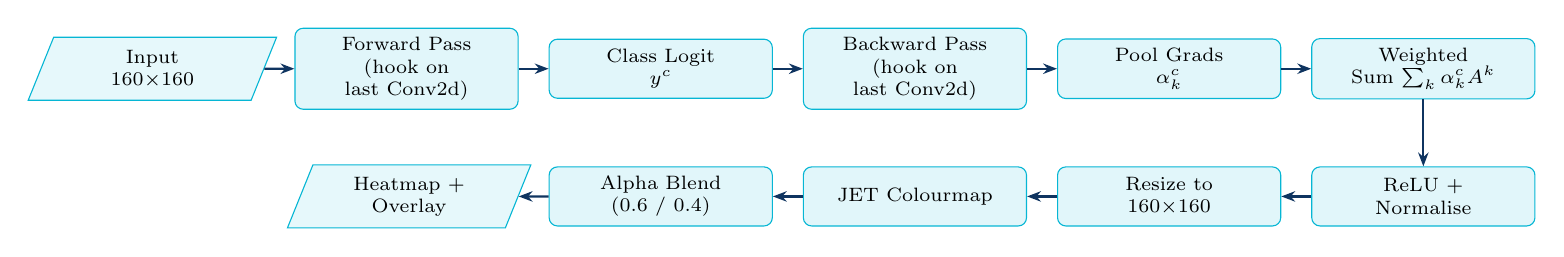
\begin{tikzpicture}[node distance=0.48cm and 0.38cm]
  \node[io, text width=2.0cm]            (img)   {Input\\$160{\times}160$};
  \node[layer, right=0.38cm of img]      (fwd)   {Forward Pass\\(hook on last Conv2d)};
  \node[layer, right=0.38cm of fwd]      (logit) {Class Logit\\$y^c$};
  \node[layer, right=0.38cm of logit]    (bwd)   {Backward Pass\\(hook on last Conv2d)};
  \node[layer, right=0.38cm of bwd]      (pool)  {Pool Grads\\$\alpha_k^c$};
  \node[layer, right=0.38cm of pool]     (wsum)  {Weighted\\Sum $\sum_k\alpha_k^c A^k$};
  \node[layer, below=0.85cm of wsum]     (relu)  {ReLU +\\Normalise};
  \node[layer, left=0.38cm  of relu]     (resize){Resize to\\$160{\times}160$};
  \node[layer, left=0.38cm  of resize]   (color) {JET Colourmap};
  \node[layer, left=0.38cm  of color]    (blend) {Alpha Blend\\(0.6 / 0.4)};
  \node[io, left=0.38cm of blend, text width=2.0cm] (out) {Heatmap +\\Overlay};

  \draw[arrow](img)--(fwd);
  \draw[arrow](fwd)--(logit);
  \draw[arrow](logit)--(bwd);
  \draw[arrow](bwd)--(pool);
  \draw[arrow](pool)--(wsum);
  \draw[arrow](wsum)--(relu);
  \draw[arrow](relu)--(resize);
  \draw[arrow](resize)--(color);
  \draw[arrow](color)--(blend);
  \draw[arrow](blend)--(out);
\end{tikzpicture}%
}
\caption{Grad-CAM computation pipeline as implemented in \texttt{generate\_gradcam()}}
\label{fig:gradcam}
\end{figure}

\subsection{Core Implementation}
\begin{lstlisting}[caption={Grad-CAM core logic (app.py)}, label={lst:gradcam}]
def generate_gradcam(model, img_tensor, class_idx):
    activations, gradients = [], []
    target_layer = get_last_conv_layer(model)   # last Conv2d in features

    fwd = target_layer.register_forward_hook(
        lambda m, i, o: activations.append(o.detach()))
    bwd = target_layer.register_full_backward_hook(
        lambda m, gi, go: gradients.append(go[0].detach()))

    out = model(img_tensor)
    model.zero_grad()
    out[0, class_idx].backward()          # backward for predicted class
    fwd.remove(); bwd.remove()

    act, grad = activations[0][0], gradients[0][0]   # (C, H, W)
    weights = torch.mean(grad, dim=(1, 2))            # global avg pool
    cam = torch.relu(sum(w * a for w, a in zip(weights, act)))
    cam = cam / (cam.max() + 1e-8)                    # epsilon guard

    cam_r   = cv2.resize(cam.numpy(), (IMG_SIZE, IMG_SIZE))
    heatmap = cv2.applyColorMap(np.uint8(255*cam_r), cv2.COLORMAP_JET)
    overlay = cv2.addWeighted(orig, 0.6,
                  cv2.cvtColor(heatmap, cv2.COLOR_BGR2RGB), 0.4, 0)
    return cv2.cvtColor(heatmap, cv2.COLOR_BGR2RGB), overlay
\end{lstlisting}

\subsection{Prediction Output}
\screenshotbox{Screenshot: Prediction Panel with Grad-CAM Overlay}{
  Insert screenshot of the \emph{Predict a Pose} section showing:
  (a) predicted class name and Sanskrit name with confidence bar,
  (b) three-column image strip: Original | Grad-CAM Heatmap | Overlay,
  (c) Top-3 horizontal bar chart and all-class probability chart (16 bars),
  (d) pose guidance card with benefits, cues, and difficulty rating.}

% ══════════════════════════════════════════════════════════════════════════
\section{Live Webcam Pose Assistance (Practical 5)}
% ══════════════════════════════════════════════════════════════════════════

In addition to single-image upload, AsanaAI provides a live webcam mode using
Streamlit's built-in \texttt{st.camera\_input}. Each captured frame is passed through
the same inference pipeline (TTA-enabled, temperature-calibrated). Predictions across
frames are smoothed using an exponential moving average (EMA) with $\alpha = 0.35$
to reduce flickering from minor pose variations:

\begin{equation}
  \hat{p}_t = \alpha\, p_t + (1-\alpha)\, \hat{p}_{t-1}
\end{equation}

A confidence threshold of 0.45 is applied; frames below this threshold show a low-confidence
warning instead of a pose name, preventing misleading feedback. The smoothed top-3
predictions and a live Grad-CAM overlay are displayed alongside the captured frame.

\screenshotbox{Screenshot: Live Webcam Mode}{
  Insert screenshot of the \emph{Live Webcam} section showing:
  (a) captured frame from webcam with pose held clearly,
  (b) smoothed prediction card with class name, Sanskrit name and EMA confidence,
  (c) live top-3 probability bars,
  (d) Grad-CAM overlay of the captured frame.}

% ══════════════════════════════════════════════════════════════════════════
\section{Model Evaluation (Practical 5)}
% ══════════════════════════════════════════════════════════════════════════

\subsection{Cached Inference Strategy}
All validation predictions are computed once and cached via Streamlit's
\texttt{@st.cache\_data}, keyed on model ID, val-loader ID, and calibration
temperature. The confusion matrix, classification report, per-class accuracy chart,
and ROC curves all share this single cached inference pass, so switching tabs
does not trigger redundant computation.

\subsection{Quantitative Metrics}

\begin{table}[H]
\centering\small
\caption{Evaluation metrics computed over the 384-image validation set (16 classes)}
\renewcommand{\arraystretch}{1.2}
\begin{tabular}{@{}lp{9cm}@{}}
\toprule
\textbf{Metric} & \textbf{Description} \\
\midrule
\rowcolor{lightblue!20} Overall accuracy &
  $(y_\text{pred} == y_\text{true}).\text{mean}()$ over all 384 val images \\
Confusion matrix &
  $16\times16$ heatmap of predicted vs.\ true class counts \\
\rowcolor{lightblue!20} Classification report &
  Per-class precision, recall, F1-score, support (scikit-learn) \\
Per-class accuracy &
  Colour-coded bars: green $\geq80\%$, orange $\geq60\%$, red $<60\%$ \\
\rowcolor{lightblue!20} ROC / AUC &
  One-vs-rest ROC curves with AUC for all 16 classes \\
\bottomrule
\end{tabular}
\end{table}

\noindent For ROC curves, each class $c$ uses its calibrated probability $p_c$ as the score
for a binary classifier (class $c$ vs.\ all others). AUC close to 1.0 indicates strong
separability. The trained model achieved a best validation accuracy of \textbf{87.6\%}
at epoch 21 out of 24 epochs.

\subsection{Evaluation Screenshots}
\screenshotbox{Screenshot: Confusion Matrix and Classification Report}{
  Insert screenshot of the \emph{Evaluation} panel, \textbf{Confusion Matrix} tab,
  showing the $16\times16$ seaborn heatmap with all class labels on both axes;
  and the \textbf{Classification Report} tab showing the styled table with
  precision, recall, F1-score, and support for each of the 16 classes.}

\screenshotbox{Screenshot: Per-Class Accuracy and ROC Curves}{
  Insert screenshot of the \textbf{Per-class Accuracy} tab (colour-coded horizontal
  bar chart for all 16 classes) and the \textbf{ROC Curves} tab (one-vs-rest curves
  for all 16 classes with AUC values in the legend).}

\subsection{Qualitative Evaluation — Grad-CAM Inspection}
Correct predictions highlight anatomically meaningful regions: the supporting leg
for Tree pose, the extended arms for Warrior, the inverted hip for Plow, and the
flat torso line for Plank. Misclassified samples typically show diffuse or
background-focused activation, which is a useful diagnostic beyond accuracy numbers.
Visually similar pose pairs (e.g., Crane vs.\ Eight-Angle) tend to have lower
confidence scores, which the calibration step reflects accurately.

% ══════════════════════════════════════════════════════════════════════════
\section{Engineering Highlights, Limitations and Conclusion}
% ══════════════════════════════════════════════════════════════════════════

\subsection{Engineering Highlights}
\begin{enumerate}[leftmargin=1.5em, label=\textbf{E\arabic*.}, itemsep=1pt]
  \item \textbf{Two-stage transfer learning} — Head warm-up then selective backbone
    fine-tuning improves accuracy and stability over end-to-end training from epoch 1.
  \item \textbf{Deep-copy best state} — \texttt{copy.deepcopy(model.state\_dict())}
    captures the best-epoch weights, avoiding reference aliasing when training continues.
  \item \textbf{Session-state guards} — Upload and training callbacks are controlled by
    \texttt{dataset\_loaded}/\texttt{trained} flags, preventing repeated side-effects.
  \item \textbf{Cached evaluation inference} — \texttt{@st.cache\_data} with model and
    loader ID keys means all metric tabs share one validation forward pass.
  \item \textbf{Temperature calibration} — Post-hoc grid search gives well-calibrated
    confidence scores; the temperature value is saved with the checkpoint.
  \item \textbf{Epsilon-guarded Grad-CAM} — Normalisation uses \texttt{max + 1e-8}
    to handle near-zero activation maps without NaN or division errors.
  \item \textbf{Palette PNG guard} — \texttt{load\_image\_rgb()} converts P-mode images
    with byte-transparency via RGBA before RGB conversion.
  \item \textbf{Webcam EMA smoothing} — Exponential moving average across captured frames
    reduces flicker and gives more stable predictions during live use.
\end{enumerate}

\subsection{Limitations}
\begin{enumerate}[leftmargin=1.5em, label=\textbf{L\arabic*.}, itemsep=1pt]
  \item Still-frame classification cannot capture movement quality, pose transitions,
    or how a pose is entered and exited over time.
  \item Ninety-six training images per class limits diversity; accuracy may drop for
    unusual lighting conditions, body types, or camera angles.
  \item Evaluation tabs require the dataset ZIP to be re-uploaded when only a checkpoint
    is loaded (single-image and webcam prediction work from checkpoint alone).
  \item Without a CUDA GPU, 24-epoch training is noticeably slower; the app shows a
    prominent CPU-only warning at startup.
\end{enumerate}

\subsection{Conclusion}
AsanaAI demonstrates a complete explainable-AI pipeline for yoga pose recognition
across 16 classes, satisfying all Practical 4 (design and implementation) and
Practical 5 (evaluation and explainability) objectives. The system combines two-stage
MobileNetV2 transfer learning, MixUp and label-smoothing regularisation, post-hoc
temperature calibration, epsilon-guarded Grad-CAM, live webcam inference with EMA
smoothing, and a full evaluation suite — all within a session-state-driven Streamlit
interface with checkpoint persistence and auto-reload.

Future improvements include: Optuna-based hyperparameter search, MediaPipe keypoint
extraction for video-based posture correction, TorchScript/ONNX export for mobile
deployment, and expanding the class set with a larger, more diverse dataset.

\end{document}